\section{Análisis del proceso actual}

A continuación se detalla cómo el Vivero Michita realiza el monitoreo y control de la gestión del consumo de agua en sus cultivos de plantas. Este proceso se ha desarrollado a partir de los datos recopilados en la entrevista realizada en el capítulo anterior. La \ref{fig:proceso_actual} detalla un análisis de este proceso, donde:

\begin{enumerate}
    \item El responsable del vivero inicia el riego de las plantas a las 8 de la mañana cada tres dias, considerando las condiciones climáticas y la cantidad de lluvia reciente.
    \item Se verifica si ha llovido lo suficiente en los últimos días:
          \begin{enumerate}[label=(\alph*)]
              \item Si ha llovido lo suficiente, no es necesario el riego durante ese día.
              \item Si no ha llovido lo suficiente, se continúa verificando la disponibilidad de agua en el arroyo.
          \end{enumerate}
    \item Se verifica si hay suficiente agua en el arroyo:
          \begin{enumerate}[label=(\alph*)]
              \item Si hay suficiente agua en el arroyo, se procede con el riego que necesita cada categoría.
              \item Si no hay suficiente agua en el arroyo, se espera a la disponibilidad de agua después del mediodía.
          \end{enumerate}
    \item El responsable procede a regar la zona que esta clasificadas por frutales, ornamentales y forestales.
    \item Después de regar la zona, el responsable realiza una inspección visual post-riego para asegurar adecuada hidratación.
    \item Se verifica si hay más zonas por regar:
          \begin{enumerate}[label=(\alph*)]
              \item Si hay más zonas por regar, se procede a regar la siguiente zona y se repite el proceso a partir del paso 4.
              \item Si no hay más zonas, se procede a planificar el siguiente riego.
          \end{enumerate}
    \item Se planifica el riego para futuras sesiones teniendo en cuenta las necesidades específicas de cada zona y las condiciones climáticas esperadas.
\end{enumerate}

\begin{figure}[h]
    \centering
    \resizebox{\textwidth}{!}{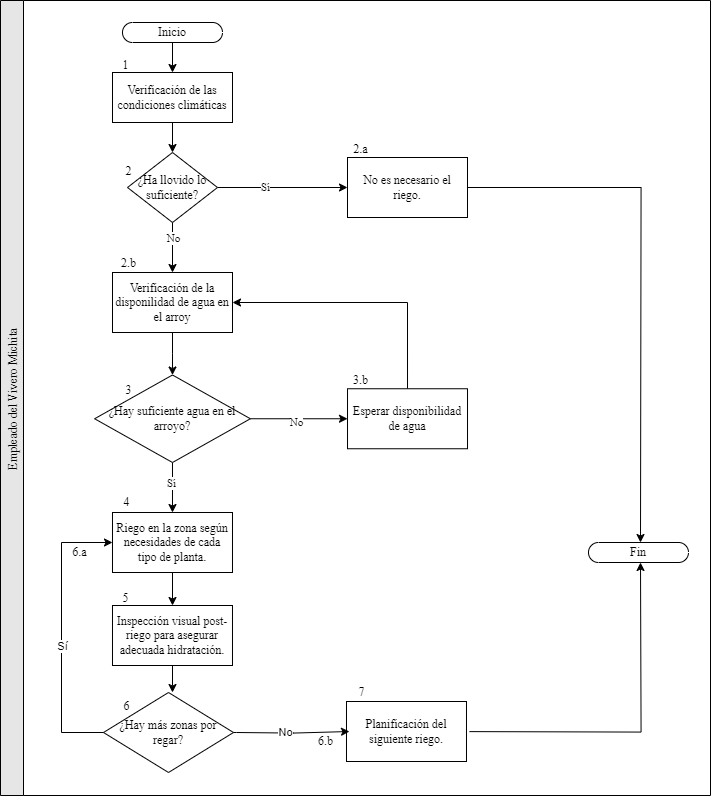
\includegraphics{resources/images/Diagrama-flujo-proceso-actual.png}}
    \caption{Diagrama de flujo del proceso actual para el monitoreo y control del riego de las plantas del Vivero Michita}\label{fig:proceso_actual}
\end{figure}



% \begin{enumerate}
%     \item Si el servicio o producto requiere de documentación adicional:
%           \begin{enumerate}[label=(\alph*)]
%               \item El responsable de la unidad solicita los documentos necesarios y los verifica, donde:
%                     \begin{enumerate}[i.]
%                         \item Si los documentos son correctos se procede con el proceso.
%                         \item Si los documentos no son correctos se finaliza el proceso.
%                     \end{enumerate}
%           \end{enumerate}
% \end{enumerate}




